\documentclass{standalone}
\usepackage{tikz}
\usetikzlibrary{arrows,shapes,positioning,shadows,trees}

\begin{document}
\begin{tikzpicture}
    \draw[-] (-3,0) -- (3,0);
    \node[fill,circle,inner sep=1pt,label=below:$O$] at (0,0) {};
    \node[fill,circle,inner sep=1pt,label=below:$-R$] at (-2,0) {};
    \node[fill,circle,inner sep=1pt,label=below:$R$] at (2,0) {};
    \draw[->] (2,0) arc (0:180:2);
    \node[label=above right:$\gamma_R$] at (2*0.6,2*0.8) {};
    \draw[->] (2*0.6 + 0.1 * 0.8, 2*0.8 - 0.1 * 0.6)-- (2*0.6,2*0.8);
\end{tikzpicture}

\begin{tikzpicture}
    \draw[-] (-3,0) -- (3,0);
    \node[fill,circle,inner sep=1pt,label=below:$O$] at (0,0) {};
    \node[fill,circle,inner sep=1pt,label=below:$-R$] at (-2,0) {};
    \node[fill,circle,inner sep=1pt,label=below:$R$] at (2,0) {};
    \draw[->] (2,0) arc (0:180:2);
    \node[label=above right:$\gamma_R$] at (2*0.6,2*0.8) {};
    \draw[->] (2*0.6 + 0.1 * 0.8, 2*0.8 - 0.1 * 0.6)-- (2*0.6,2*0.8);
    \node[fill,circle,inner sep=1pt,label=right:$i$] at (0,1) {};
\end{tikzpicture}

\begin{tikzpicture}
    \draw[-] (-4,0) -- (4,0);
    \node[fill,circle,inner sep=1pt,label=below:$O$] at (0,0) {};
    \node[fill,circle,inner sep=1pt,label=below:$-R$] at (-3,0) {};
    \node[fill,circle,inner sep=1pt,label=below:$R$] at (3,0) {};
    \draw[->] (0,0) -- (0,2.5);
    \node[fill,circle,inner sep=1pt,label=right:$i\pi$] at (0,1) {};
    \node[fill,circle,inner sep=1pt,label=above right:$2i\pi$] at (0,2) {};
    \draw[->] (3,0) -- (3,1);
    \draw[-] (3,1) -- (3,2);
    \node[label=above right:$\gamma_1$] at (3,1) {};
    \draw[->] (3,2) -- (2,2);
    \draw[-] (2,2) -- (-3,2);
    \node[label=above right:$\gamma_2$] at (2,2) {};
    \draw[->] (-3,2) -- (-3,1);
    \draw[-] (-3,1) -- (-3,0);
    \node[label=above left:$\gamma_3$] at (-3,1) {};
\end{tikzpicture}

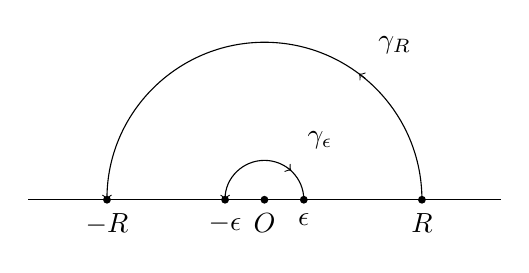
\begin{tikzpicture}
    \draw[-] (-3,0) -- (3,0);
    \node[fill,circle,inner sep=1pt,label=below:$O$] at (0,0) {};
    \node[fill,circle,inner sep=1pt,label=below:$-R$] at (-2,0) {};
    \node[fill,circle,inner sep=1pt,label=below:$R$] at (2,0) {};
    \draw[->] (2,0) arc (0:180:2);
    \node[label=above right:$\gamma_R$] at (2*0.6,2*0.8) {};
    \draw[->] (2*0.6 + 0.1 * 0.8, 2*0.8 - 0.1 * 0.6)-- (2*0.6,2*0.8);
    \node[fill,circle,inner sep=1pt,label=below:$-\epsilon$] at (-0.5,0) {};
    \node[fill,circle,inner sep=1pt,label=below:$\epsilon$] at (0.5,0) {};
    \draw[->] (0.5,0) arc (0:180:0.5);
    \node[label=above right:$\gamma_\epsilon$] at (0.5*0.6,0.5*0.8) {};
    \draw[->] (0.5*0.6,0.5*0.8) -- (0.5*0.6 + 0.05*0.8, 0.5*0.8 - 0.05*0.6);
\end{tikzpicture}
\end{document}